\chapter{Discussion, future work \& conclusions}
\lhead{Chapter 5 \emph{Discussion, future work \& conclusions}}
\label{chap:5}
%\autoref{chap:5}

\bigskip
\section{Evaluation \& discussion}
\bigskip

In this section the experiments and results presented in the previous chapter will be evaluated. One way to assess the results of this software is to compare them with the equivalent information that has been published. For this reason, the results that were presented are concerning satellites or constellations that are well documented and information regarding the revisit time of them can be found.

To start with the experiments on the single satellites and as it can be seen in Figure \ref{revisit_time_Sentinel2A}, the average revisit time of Sentinel-2A at equator is almost 10 days, which can be confirmed from the official ESA's documentation \footnote{\label{Sentinel2_source}\textit{Available at: https://sentinel.esa.int/web/sentinel/missions/sentinel-2 (Accessed November 20, 2020)}}. Additionally, it can be noticed that there are certain longitude cells from which the satellite does not pass. Since Sentinel-2A is in a sun-synchronous orbit, it means that after a certain period of time the orbit repeats and it can also happen that the satellite never crosses from some areas in the globe. The same characteristics and a revisit time of 10 days is also true for its twin satellite, Sentinel-2B.

\bigskip
In the same manner, the average revisit time of Sentinel-3A (Figure \ref{revisit_time_Sentinel3A}) is less than 2 days, which can be also validated \footnote{\label{Sentinel3A_source}\textit{Available at: https://sentinel.esa.int/web/sentinel/user-guides/sentinel-3-synergy/coverage (Accessed November 20, 2020)}}. The reason behind this rapid revisit time at the equator is the large swath width of its sensors, which is of 1270 km. This means that the larger the swath width of a sensor is, the larger is the area that is captured and thus the quicker the revisit time is.

It can be also noticed from the Figure \ref{revisit_time_Sentinel3A} that every longitude cell has information about the revisit time, which means that the satellite captures images along all the equatorial cells. On the one hand, this can be possibly explained by the fact that there is overlapping coverage between the adjacent orbits. For examining this case, the angular distance $\Delta \lambda$ of successive ascending equator crossings should be calculated (Equation \ref{delta_lambda}), once the period of the satellite has been found. So, for the Sentinel-3A the period is $T \sim 6056 \text{ [sec]}$ or $T \sim 101 \text{[ min]}$ and thus the $\Delta \lambda$ between the adjacent orbits is $\Delta \lambda \sim 25\text{ [degrees]}$. This can also be verified by plotting its groundtrack (see Figure \ref{Sentinel_3A_delta_lambda}). Finally, by converting the $\Delta \lambda$ from degrees to kilometers it is concluded that there is not overlapping coverage between the adjacent orbits, since the $\Delta \lambda \sim 2775\text{ [kilometers]}$ and swath width is 1270 km. All in all, in this revisit time calculation of Sentinel-3A it could be argued that even though there is not overlapping coverage between successive orbits as proved, the satellite is able to capture images along all the equatorial line. 

\begin{figure}
\centering
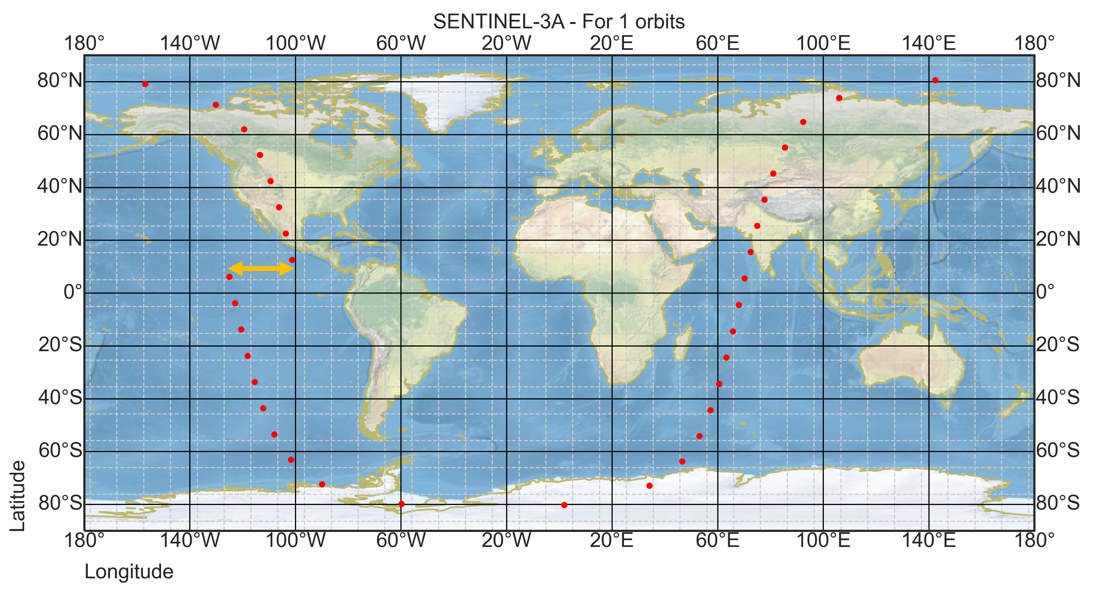
\includegraphics[width=0.9\textwidth]{Images/Sentinel_3A_delta_lambda.png}\caption{The groundtrack of Sentinel-3A for one orbit. The yellow arrow indicates the angular distance $\Delta \lambda$ of successive ascending equator crossings. As it can also be validated from the equation \ref{delta_lambda}, it is approximately 25 degrees.}
\label{Sentinel_3A_delta_lambda}
\end{figure}

\bigskip

The evaluation of the results of the two other presented single satellite's calculations of the revisit time along the equator comes from the JACIE's (Joint Agency Commercial Imagery Evaluation) group report of 2019 \cite{Christopherson}. To be more exact, in Figure \ref{revisit_time_of_ALSAT 1B} can be seen that the average revisit time at the equator is around 5 days, which can also be confirmed in the above-mentioned report. Similarly, the revisit time at the equator for the satellite GOMX-4A has been also found to be 5 days.

\bigskip
As for the evaluation concerning the revisit time of multiple satellites or constellations, it was first important to make sure that all the involved satellites have the same starting epoch for their propagation. For this reason, the groundtrack of one orbit for the Sentinel-2 constellation was presented. In Figures \ref{groundtrack_Sentinel-2A}, 
\ref{groundtrack_Sentinel-2B} it can also be verified the fact that those twin satellites are phased at 180 degrees to each other.

The average revisit time at the equator for the Sentinel-2 constellation is around 5 days, as it can be seen in Figure \ref{revisit_time_of_SENTINEL-2A_SENTINEL-2B}, which can be validated by ESA's documentation \footnote{\label{Sentinel2_source}\textit{Available at: https://sentinel.esa.int/web/sentinel/missions/sentinel-2 (Accessed November 20, 2020)}}. Similarly, the revisit time for the Sentinel-1 constellation is 3 days as seen in Figure \ref{revisit_time_of_SENTINEL-1A_SENTINEL-1B}, whose validity can be also checked \footnote{\label{Sentinel1_source}\textit{Available at: https://sentinel.esa.int/web/sentinel/user-guides/sentinel-1-sar/revisit-and-coverage (Accessed November 20, 2020)}}.

\bigskip
Regarding the first experiment of finding the position of a new satellite, which can achieve a more frequent revisit time together with a group of other satellites, namely the Sentinel-2 constellation, the Figure \ref{revisit_time_ofdoubleaxis_SENTINEL-2A_SENTINEL-2B_Example-satellite} was created. As can be seen, the overall revisit time of the three satellites was calculated also at the positions of Sentinel-2A and 2B individually. For those positions, indicated with green lines, the overall revisit time was found to be close to 5 days. The reason behind is that the Example-satellite in these positions is co-located with one of the two other satellites, which fact does not result in reducing the revisit time of the one achieved only by the Sentinel-2 constellation. The revisit time of 5 days in those positions can also be validated from the Figure \ref{revisit_time_of_SENTINEL-2A_SENTINEL-2B}, in which the average revisit time at equator of the Sentinel-2 satellites is shown.

Additionally, it was noticed that although the influence of the new's satellite mean anomaly change in the combined revisit time brings a large reduction rate, of abound 35\%, the differences of the revisit time between the various positions in the orbital plane are not large (Figure \ref{revisit_time_ofdoubleaxis_SENTINEL-2A_SENTINEL-2B_Example-satellite}). Therefore, placing a new satellite in the same orbital plane as of the other satellites will bring a significant reduction in the revisit rate independently of the exact position in the orbital plane. Nevertheless, attention needs to be paid to not placing a new satellite in the same position as another existing satellite is.  

\bigskip
The second experiment pertained to the investigation of the overall revisit time when the altitude of the new satellite varies. For this case, several examples were presented in Chapter \ref{chap:4} and in each of those the new satellite is placed in a different position in the orbital plane. More specifically, as can be seen in Figures \ref{revisit_time_ofdoubleaxisaltitude_SENTINEL-2A_SENTINEL-2B_Example-satellite_50deg}, \ref{revisit_time_ofdoubleaxisaltitude_SENTINEL-2A_SENTINEL-2B_Example-satellite_180deg}, \ref{revisit_time_ofdoubleaxisaltitude_SENTINEL-2A_SENTINEL-2B_Example-satellite_330deg}, in all those example cases the same behavior can be noticed. The most frequent revisit time is close to the altitude that the rest of the satellites are located and the revisit time becomes less often the further away the satellite is located from this altitude. As for the reduction of the revisit time that can be seen in the right-side y-axis of the Figures, it should be mentioned that is the same compared with the reduction rates from the previous experiment when varying the position in the orbital plane.
% The influence of the altitude change in the revisit time is that it is always drifting with respect to the other. --> THE MORE YOU GO AWAY FROM THAT ALTITUDE, THE LESS PRONOUNCED WILL BE THE DIFFERENCE COMPARED TO THE DIFFERENCES FROM THE MEAN ANOMALY'S CASE.

The same experiment of varying the altitude of a new satellite when it is added in the calculation of the overall revisit time was implemented for the group of the 37 Flock-3P satellites (Figure \ref{revisit_time_ofdoubleaxisaltitude_Flocks}). As mentioned above, the revisit time is drifting with respect to the altitude change, with the lowest point being in the mean altitude of the rest of the satellites. Despite that, in this case in which the number of engaged satellites is as large as of 37, the reduction of the revisit time as can be seen in Figure, is around 2-3\%. In comparison with the reduction of the revisit time when a satellite is added to a smaller group of satellites (\sim 34\% e.g. Figure \ref{revisit_time_ofdoubleaxisaltitude_SENTINEL-2A_SENTINEL-2B_Example-satellite_50deg}), this rate is significantly lower, which indicates that by adding one satellite in an already large group of satellites does not contribute much in the α a rapider revisit time

\bigskip

% Combination of all Flocks (not even Skysats) and the revisit time close.. imagine that since the calculation is at equator and the orbits are near-polar, at the equator is the less frequent revisit time.


\bigskip
\subsection{Strengths \& contribution of thesis}
\bigskip

It should be also noted that it is not always easy to validate the results concerning the revisit time of a satellite. One of the reason behind of it is that 

The importance of this software is that a user can find out the revisit time Many satellite operators either do not announce the revisit time, or when they do it is not specified in which latitude and finally some of them measure the revisit time at a reference altitude (when the satellites of the fleet orbit on a different altitude).
%revisit time of Skysat is ~4-5 days (it is measured with reference altitude 500km. It is written in their pdf).  Companies say “reference altitude”. However the orbit of the satellite does not have this altitude. Source: https://assets.planet.com/docs/Planet_Combined_Imagery_Product_Specs_letter_screen.pdf 

A user can find the revisit time from multiple satellites..

Prioritization of the missions based on the added value in the society. So say that this work has helped into this direction...

% It is important that a clear definition and way of computing the revisit time with the results of some renowed satellites and constellation has been created. The announced information and revisit time that the satellites have from companies and institues are vague and not clear. Which assumptions have been made etc...

\bigskip
\subsection{Limitations} %Problems
\bigskip

The main input of this application, as well as a source that can affect the performance of the software is the accuracy of the TLE of the satellites.

"The satellites elements go rapidly out of date. The "epoch" of the element set should be in a recent date. The older it is the more inaccurate the parameters might be. Since the application refers to the future, it is necessary to have the most recent TLE. The providers like Clestrak update them almost daily. A TLE set can predict the position of a satellite approximately for  two weeks into the future.

Another issue that arises with the TLE's use is (maybe shift this first).
"It should be noted that when using TLE sets from NORAD, it is important to realize that not just any prediction model can be used. The elements of NORAD TLEs are mean values, which were obtained by removing periodic variations in a particular way (SGP4 way). To get the most precise prediction results it is important that these variations will be reconstructed in the same way as they were removed. When the SGP4 model is used, these optimal results are achieved. However, in this application, since high precision is not necessary... It general periodical SGP model gives approximately 1 km accuracy over a short (ca few days) propagation time. (VALLADO)
The exact process for updating TLE is not well known with every detail. Essentially, observations are collected several times a day at the Joint Space Operations Center (JSPOC) operated by the US Air Force Space Command (AFSPC). Once, the observation pass through an initial association and verification pass, they are passed to the orbit determination operation using SGP4 and numerical techniques (cite: TLE_Vallado)
The satellite observations processes are executed in an automated fashion. There is no knowledge of maneuvers before or after the current time of OD generation. During the processing, the presence of maneuvers inflates the uncertainty of any estimate, but because the TLEs are delivered without a covariance, there is little way of knowing if there is increased uncertainty in a particular TLE from the previous estimates. Indeed as it was investigated by Intelsat, The JSPOC has no knowledge of the satellite owner maneuvers and naturally the TLE of the maneuvering satellites have large errors. (cite: TLE_Vallado)


% From the plot of Investigation.. we see that the revisit time of satellites, which are part of constellations can vary significantly. We might see that the satellites, which have wider swath width have shorter revisit time. However, the revisit time is connected with multiple parameters. BY KRAMER: If we want quick revisit times (like “daily” and not some like 16 days) of a particular area, we need LEO orbits at HIGHER altitudes (say 3000 km) providing considerably wider ground swaths, but with coarser resolution. (Kramer_2002)

%The discussion will consist of argumentation. In other words, you investigate a phenomenon from several different perspectives. To discuss means to question your findings, and to consider different interpretations. Here are a few examples of formulations that signal argumentation:
%
%On the one hand … and on the other …
%However …
%… it could also be argued that …
%… another possible explanation may be …

% Maybe add sth about the duration of the simulations.. about the resonance?! (I had written some stuff at the beginning of the 4th Chapter) "Some satellites hit resonances. Needs more careful investigation.. Some satellites have longer revisit time than others (from the same constellation). I am not sure if I want to say this :)


\bigskip
\section{Future work}
\bigskip

%* Info about the tilt angle
%* Extend to other fields - Communication etc
%++ what can be done more? Finally, more complex sensor shapes could be investigated and dierent projection geometries could be studied to ensure accuracy of the method at higher target latitudes.
%++ Calculation of revisit time metrics considering
%time of night/day or lighting conditions would also enable
%particular application for optical Earth observation
%sensors. (mallon min to anafereis. Einai polu sxetiko me tin ergasia... Mipos na to eixa kanei?)

Future work: the database should be connected to a TLE provider and the TLE of each satellite should be updated.

Use the method of Lemmens, Krag (se sxolio in master_thesis file in LaTeX), which detects orbital maneuvers of satellite by checking the consistency between arbitrary two-line element sets of the same object. In this way, the non-natural anomalous events of orbits can be foud and the TLE set that produced this kind of orbit can be left out from the further calculations until is discovered whether this new presented orbit is a permanent one.

% Check comments on "Scientific questions.doc" (about revisit time, inclination, swath width, altitude etc)

% !! Parallel computing methods can be used to improve this performance significantly by increasing the number of computations which can be performed in a given period of time.

% Place an index at the "international designator" in the PostgreSQL for faster searching. So far is not needed.

% If the software wants to be expanded in other areas not only near-polar orbits EO.. then the coverage along the equator needs to be computed based on the inclination angle (as well!) and the swath width. Check image of swath_width_groundtrack.png)

\bigskip
\section{Conclusions}
\bigskip

Revisit time VS repeat period. 1st overlapping gaps + swath width (characteristic of sensor) --> Importance of applications

Prioritization of the missions based on the added value in the society. So say that this work has helped into this direction...

%Who will be helped with this work? It will give the incentives etc etc buuuut These plots on their own and the supporting data can provide valuable reference for Earth observation system designers in the early phases of a mission development lifecycle. (By Crisp_2018 p.10) 

First, the revisit time is latitude dependent! Since we find the revisit time at the equator and we have near-polar orbits, the equator has the less frequent revisit time.

From the experiment of the whole Flock constellation it seems that rapider revisit times can be clearly achieved with the cooperation and ...

% Probably when ther is an already large constellaiton, a single satellite doesn't add basically any significant value. (this is what Vitali expects). --> Check the revisit rate of the extra satellite in the example of Flocks. YES

It was noticed that the rapider revisit rates can be achieved when adding a satellite in the same orbital plane and not placing it in a higher or lower orbital planes. However, if the orbital plane has already a large number of satellites, then the option of changing the altitude of the new satellite is inevitable in order to avoid the risk of conjunctions between the other satellites. All the same, in such case the altitude change of the new satellite should not exceed five km.